\subsection{Compiler Design}
\label{sec:CompilerDesign}

As both the \lexer{} and the \parser{} are generated by third party tools, these will
not be covered, but a full table of the tokens and the
production rules can be found in appendix~\ref{sec:appA} and \ref{sec:appB}. To best
understand the design of the \static, its components: the type checker and the borrow
checker, as well as the \codeGen{}, requires an understanding of
the visitor pattern, as well as the structure of the \ast{} of a typical \lang{}
program.

\subsubsection{Understanding the AST}
\label{sec:AST}

The \ast{} of a typical \lang{} program can typically be divided into three
sections; the program layer, the function layer and the expression layer (see
figure~\ref{fig:astStruct}). Each node in the \ast{} correspond one-to-one with a
type of expression in \lang{} and will hereafter be refered to as nodes or
expressions. 

\newpage 

\begin{figure}[ht]
  \centering
  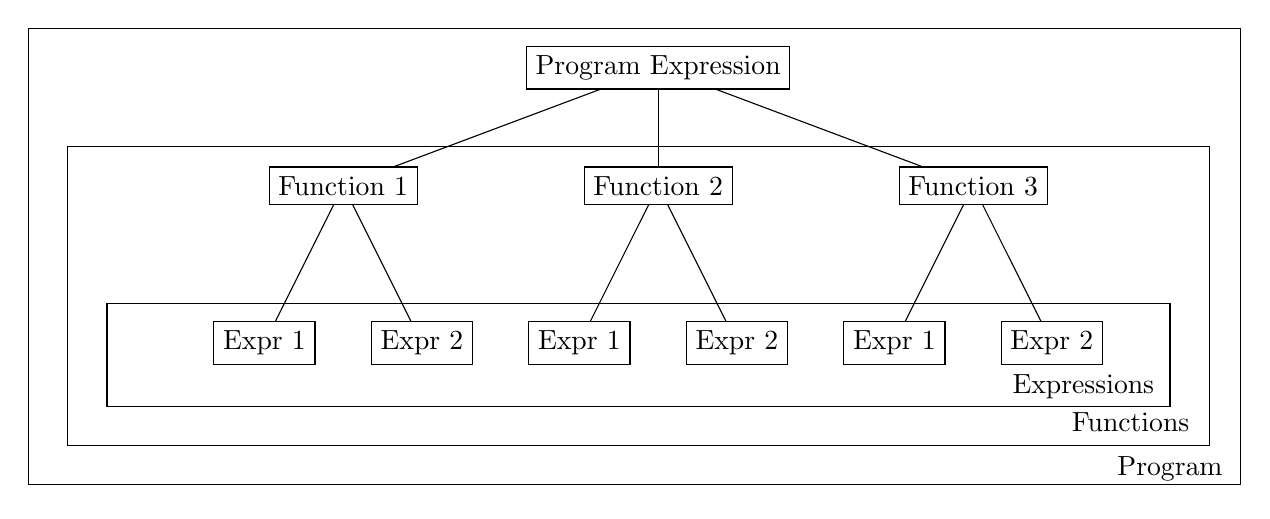
\begin{tikzpicture}
    \node[draw] (program) at (0, -0.5) {Program Expression};

    \def\functions{{Function 1}, {Function 2}, {Function 3}};
    \def\instructions{{Expr 1}, {Expr 2}}

    \foreach \fun [count=\i] in \functions {

      \pgfmathtruncatemacro{\x}{(-8 + (\i)*4)};
      \node[draw] (func\i) at (\x, -2) {\fun};
      \draw[] (program) -- (func\i); 

      
    }

    \node[draw] (int1) at (-5,-4) {Expr 1};
    \node[draw] (int2) at (-3,-4) {Expr 2};

    \draw[] (func1) -- (int1);
    \draw[] (func1) -- (int2);
    
    \node[draw] (int3) at (-1,-4) {Expr 1};
    \node[draw] (int4) at (1,-4) {Expr 2};

    \draw[] (func2) -- (int3);
    \draw[] (func2) -- (int4);
    
    \node[draw] (int5) at (3,-4) {Expr 1};
    \node[draw] (int6) at (5,-4) {Expr 2};

    \draw[] (func3) -- (int5);
    \draw[] (func3) -- (int6);
 
    \draw[] (-8,0) rectangle (7.4,-5.8);
    \draw[] (-7.5,-1.5) rectangle (7,-5.3);
    \draw[] (-7,-3.5) rectangle (6.5,-4.8);

    \node[] (programBox) at (6.5, -5.6) {Program};
    \node[] (functionBox) at (6, -5) {Functions};
    \node[] (instructionBox) at (5.4, -4.55) {Expressions};
  \end{tikzpicture}
  \caption{\ast{} for \lang{} showing how a typical program is structured after
  being parsed by the \lang{} parser. Each expression node, can then be further
subdivided until reaching the leafs of each branch which corresponds to terminal
expressions.}
  \label{fig:astStruct}
\end{figure}

It is this structure on which the \typeChecker, the \borrowChecker, and the
\codeGen{} will operate to produce an object file which the \gcc{} can turn into an
excutable file. The use of the visitor pattern (see section~\ref{sec:VisitorDesign})
is specifically used to facilitate a depth first, left to right traversal of the
\ast{} to do type checking, borrow checking and code generation.

This ensures the code is analyzed in the same order in which it appears in the
source code.

\subsection{Visitor Pattern}
\label{sec:VisitorDesign}

As can be seen on figure \ref{fig:CompilerProcess}, several steps in the compilation process acts on the AST, with semantic analysis containing both type- and borrow checking.
It would be desirable to have a unified way of traversing the structure for all the different steps. The immediate and naive solution would be to implement the different algorithms into the tree nodes directly. This approach has the appeal of making it easy to add new nodes. It does, however, make it difficult to add additional functionality to the compiler, as every addition requires a modification of every expression class. A solution to this great coupling is to use the visitor design pattern.

The visitor pattern separates algorithms from an object structure by implementing a 'visitor' class which can traverse the tree and perform the correct operations on each node. This allows for additional functionality to be added, without modifying the existing tree (thus following the open-closed principle). As long as every node implements an 'accept' function, new visitors can be added without the need for altering the expression classes at all. 

\begin{figure}
\includegraphics[width=\textwidth]{02-Body/Images/VisitorClassDiag.png}
\caption{Class diagram for Visitor Pattern}
\label{fig:VisitorClassDiagram}
\end{figure}

\subsubsection{Type Checker}

The \typeChecker{} 

\newpage

\subsection{Borrow Checker}
\label{sec:BorrowCheckerImpl}




\subsection{Code Generator}
\label{sec:CodeGenImplement}
Implementation inspired by \cite{LLVMTutorial}
